%----------------------------------------------------
% Setup Beamer
%----------------------------------------------------
\documentclass[hyperref={colorlinks=true}]{beamer}

%----------------------------------------------------
% Packages to use
%----------------------------------------------------
\input{../packages.sty}

%----------------------------------------------------
% Setup Theme
%----------------------------------------------------
\input{../theme.sty}

%----------------------------------------------------
% Table of Contents at each section transition
%----------------------------------------------------

\AtBeginSection[]
{
   \begin{frame}
       \frametitle{Outline}
       \setcounter{tocdepth}{2}
       \tableofcontents[currentsection]
   \end{frame}
}

%----------------------------------------------------
% Colors
%----------------------------------------------------
\input{../mycolors.sty}

%----------------------------------------------------
% Style, formatting, and new commands
%----------------------------------------------------
\newcommand{\CourseYear}   {2024}
\newcommand{\CanvasURL}    {https://canvas.uchicago.edu/courses/58627}
\newcommand{\CanvasLink}   {\href{\CanvasURL}{\CanvasURL}}
\newcommand{\GitHubURL}    {https://github.com/UChicagoPhysics/PHYS250}
\newcommand{\GitHubLink}   {\href{\GitHubURL}{\GitHubURL}}
\newcommand{\PlatformURL}  {https://binderhub.pile.uchicago.edu/}
\newcommand{\PlatformLink} {\href{\PlatformURL}{\PlatformURL}}
\newcommand{\PiazzaURL}    {https://canvas.uchicago.edu/courses/58627/discussion\_topics}
\newcommand{\PiazzaLink}   {\href{\PiazzaURL}{\PiazzaURL}}
\input{../newcommands.sty}
\input{../EandMcommands.sty}

%----------------------------------------------------
% Set paths for plots and images
%----------------------------------------------------
\input{../paths.sty}

%----------------------------------------------------
% SETTINGS FOR THIS LECTURE
%----------------------------------------------------
\newcommand{\lecnum }  {Lecture 12}
\newcommand{\lecdate}  {November 7, 2024}
\newcommand{\topic}    {Fourier Transforms: Discrete, Fast, and Practical}

%-----------------------------------------------------------------------------------------
% Title: [Column]{Title}
%-----------------------------------------------------------------------------------------
\title[PHYS 250 (Autumn 2024) -- \lecnum]{\topic}

%-----------------------------------------------------------------------------------------
% SubTitle: [Column]{Subtitle}
%-----------------------------------------------------------------------------------------
\subtitle{PHYS 250 (Autumn 2024) -- \lecnum}

%-----------------------------------------------------------------------------------------
% Author: [SubAuthor]{Author}
%-----------------------------------------------------------------------------------------
\author[D.W.~Miller]{David Miller}

%----------------------------------------------------
% Institute: [SubInst]{Institute}
%----------------------------------------------------
\institute[EFI, Chicago] 
{
  Department of Physics and the Enrico Fermi Institute\\
  University of Chicago
}

%----------------------------------------------------
% Institute: [SubInst]{Institute}
%----------------------------------------------------
\date[\lecdate]{\lecdate}

\subject{PHYS 250 Lecture}

\begin{document}

%==========================================================================================
% TITLE PAGE
%==========================================================================================

{
\begin{frame}
  \titlepage
\end{frame}
}

%==========================================================================================
\section[Reminders]{Reminders}
%==========================================================================================

%-----------------------------------------------------------------------------------------
\subsection[Reminders from Lecture 13]{Reminders from Lecture 13}
%-----------------------------------------------------------------------------------------

\begin{frame}%[shrink=10]
  \frametitle{Reminders from last time}

  We left off discussing details of our discrete Fourier transform and how we might speed it up.
  
  \vspace{0.3cm}
  
  \begin{ucblock}{PDEs and Fourier Series}
    \begin{itemize}
      \item \bluebf{Fourier Series \ra\ Fourier Transforms} 
      \begin{itemize}
        \item We discussed how we can move to a continuous function definition of the expansion over a basis of functions
        \item We then broke this down into discrete steps and obtained the \alertbf{Discrete Fourier Transform}
      \end{itemize}
      \item \bluebf{Issues encountered:} 
      \begin{itemize}
        \item We realized that there is an issue related to the finite sampling of a function: \alertbf{aliasing}
        \item Began to break down the Fourier transform even further for a \alertbf{fast} implementation
      \end{itemize}
    \end{itemize}
  \end{ucblock}
  
  \mysp
  
  Today we will discuss the evolution towards the \alertbf{FFT}, some of the practical limitations, and specific real-world (scientific and otherwise!) examples of using FFT's!

\end{frame}

%-----------------------------------------------------------------------------------------


\begin{frame}%[shrink=10]
  \frametitle{Square wave Fourier series}

  We already saw how we can break down a ``simple'' function into its components:

  \mysp

  \pgfplotsset{width=\textwidth,compat=1.6}

  \centering

  \begin{tikzpicture}
    \begin{axis}[
        set layers=standard,
        domain=0:10,
        samples y=1,
        view={40}{20},
        hide axis,
        unit vector ratio*=1 2 1,
        xtick=\empty, ytick=\empty, ztick=\empty,
        clip=false
    ]
    \def\sumcurve{0}
    \pgfplotsinvokeforeach{0.5,1.5,...,5.5}{
        \draw [on layer=background, gray!20] (axis cs:0,####1,0) -- (axis cs:10,####1,0);
        \addplot3 [on layer=main, blue!30, smooth, samples=101]
          (x,####1,{sin(####1*x*(157))/(####1*2)});
        \addplot3 [on layer=axis foreground, very thick, blue,ycomb, samples=2]
          (10.5,####1,{1/(####1*2)});
        \xdef\sumcurve{\sumcurve + sin(####1*x*(157))/(####1*2)}
    }
    \addplot3 [red, samples=200] (x,0,{\sumcurve});
    \draw [on layer=axis foreground]  (axis cs:0,0,0) -- (axis cs:10,0,0);
    \draw (axis cs:10.5,0.25,0) -- (axis cs:10.5,5.5,0);
    \end{axis}
  \end{tikzpicture}
  
  \mysp
  
  So let's figure out how to use this to its full capacity!

\end{frame}


%==========================================================================================
\section[DFT to FFT]{DFT to FFT}
%==========================================================================================

%-----------------------------------------------------------------------------------------

\begin{frame}%[fragile,shrink=15]
  \frametitle{Discrete Fourier Transforms (I)}

  If $\hat{f}(\omega)$ or $f(t)$ are known analytically or numerically, the Fourier transform integrals can be evaluated using the integration techniques studied earlier. 
  
  \mysp \pause
  
  In practice, the signal $f(t)$  is measured, or \alertbf{sampled} at just a finite number $N$ of times $t$, and these are what we must use to approximate the transform. 
  
  \mysp \pause
  
  The resultant \alertbf{discrete Fourier transform (DFT)} is an approximation both because the signal is not known for all times and because we integrate numerically.
  
  \mysp \pause
  
  Once we have a discrete set of transforms, they can be used to reconstruct the signal for any value of the time. 
  
  \mysp \pause
  
  In this way the \bluebf{DFT can be thought of as a technique for interpolating, compressing, and extrapolating data}.
  
\end{frame}

%-----------------------------------------------------------------------------------------

\begin{frame}%[fragile,shrink=15]
  \frametitle{Discussion}

  \centering \Large \bluebf{Do you see any issues with this ``sampling''? }
  
  \pause
  
  \begin{figure}
    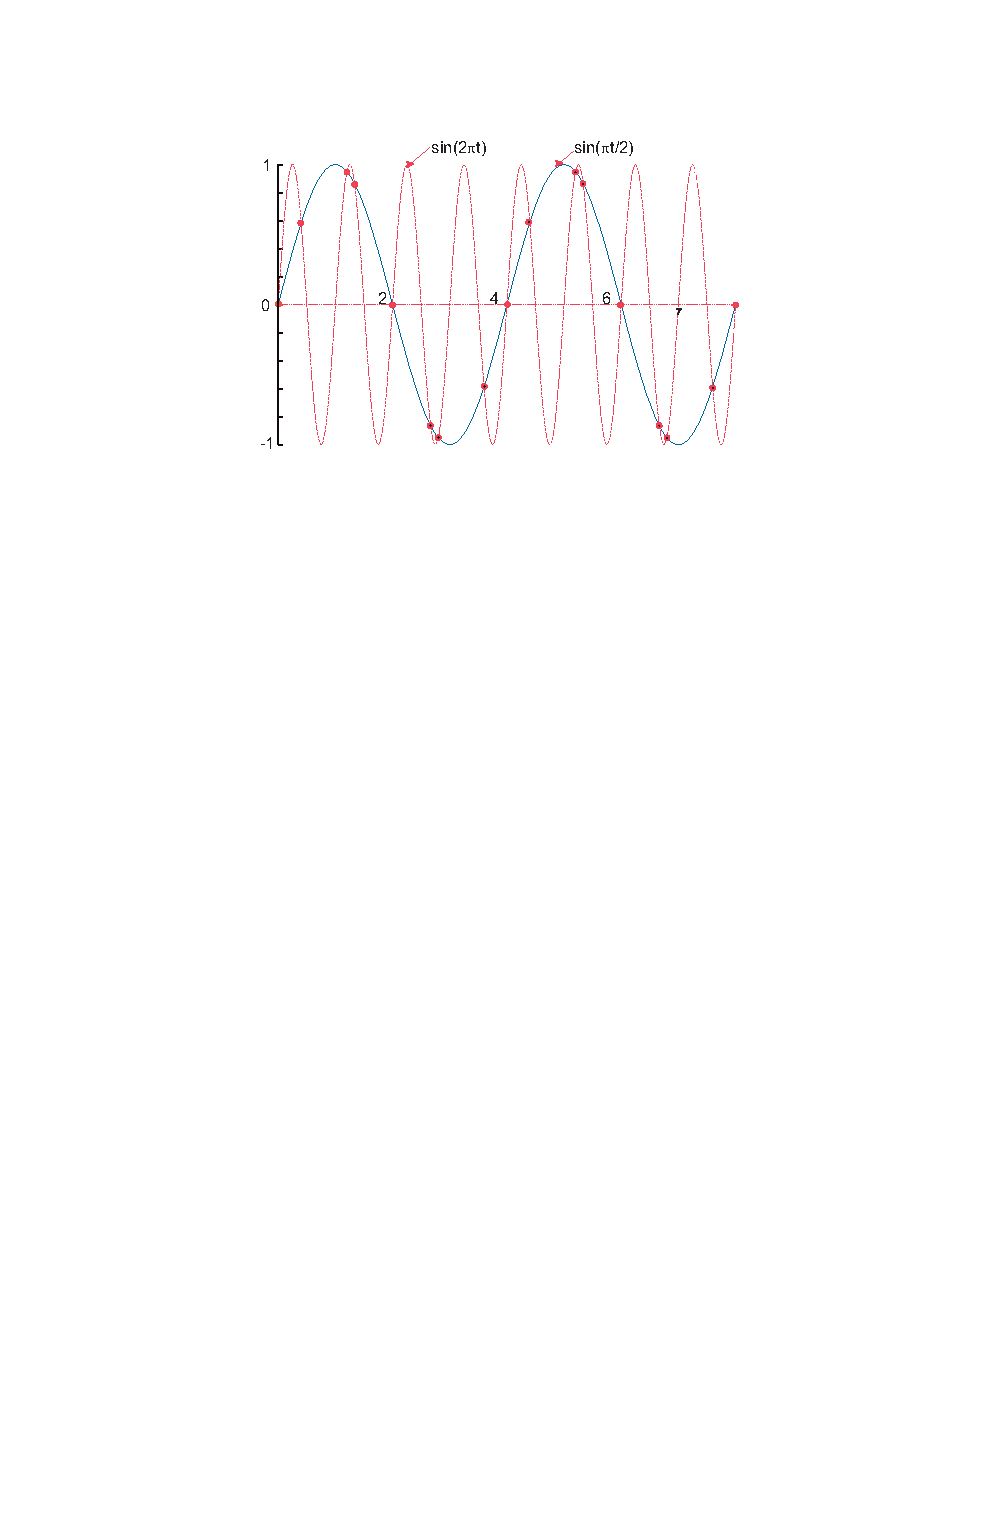
\includegraphics[width=0.9\columnwidth]{Aliasing.pdf}
  \end{figure}
  
\end{frame}

%-----------------------------------------------------------------------------------------

\begin{frame}%[fragile,shrink=15]
  \frametitle{Discrete Fourier Transforms (II)}

  The DFT algorithm results from evaluating the integral not from $-\infty$ to $+\infty$ but rather from time $0$ to time $T$ over which the signal is measured, and from approximating the integration of the integral by computing a discrete sum:
  
  \begin{eqnarray}
    \hat{f}(\omega_n) &=& \frac{1}{\sqrt{2\pi}} \int_{-\infty}^{\infty} f(t)   e^{-i\omega_n t}   dt \\
                 &\simeq& \frac{1}{\sqrt{2\pi}} \int_{0}^{T}            f(t)   e^{-i\omega_n t}   dt \\
                 &\simeq& \frac{1}{\sqrt{2\pi}} \sum_{k=1}^{N}     h \, f(t_k) e^{-i\omega_n t_k} \qquad (h\equiv\mathrm{stepsize}) \\
                 &\simeq& \frac{h}{\sqrt{2\pi}} \sum_{k=1}^{N}          f_k    e^{-2\pi i k n/N}     \\
    \hat{f}_n \equiv \frac{\hat{f}(\omega_n)}{h} &=& \frac{1}{\sqrt{2\pi}} \sum_{k=1}^{N}  f_k  e^{-2\pi i k n/N}  
  \end{eqnarray}
  
\end{frame}

%-----------------------------------------------------------------------------------------

\begin{frame}%[fragile,shrink=15]
  \frametitle{Discrete Fourier Transforms (III)}

  We then need the inverse as well, which we can obtain with $d\omega \rightarrow 2\pi/Nh $ we invert the $\hat{f}_n $
      
  \begin{eqnarray}
    f_k &=& \frac{1}{\sqrt{2\pi}} \sum_{n=1}^{N} \frac{2\pi}{Nh}  \hat{f}_n  e^{i\omega_n t}  
  \end{eqnarray}
  
  Once we know the $N$ values of the transform $\hat{f}_n$, we can use this expression to evaluate $f(t)$ for any time $t$. The frequencies $\omega_n$ are determined by the number of samples taken and by the total sampling time $T = N h$ as
  
  \begin{equation}
    \omega_n = n\frac{2\pi}{Nh}
  \end{equation}
  
  Clearly, the larger we make the time $T = Nh$ over which we sample the function, the smaller will be the frequency steps or resolution. Accordingly,if you want a smooth frequency spectrum, you need to have a small frequency step $2\pi/T$.
  
\end{frame}

%-----------------------------------------------------------------------------------------

\begin{frame}%[fragile,shrink=15]
  \frametitle{Discrete Fourier Transforms (IV)}

  Lastly, we can simplify this expression to yield a clear computational approach:
      
  \begin{eqnarray}
    f_k       &=& \frac{\sqrt{2\pi}}{N} \sum_{n=1}^{N} Z^{-nk}\hat{f}_{n} \qquad (Z=e^{-2\pi i/N}) \\
    \hat{f}_n &=& \frac{1}{\sqrt{2\pi}} \sum_{k=1}^{N} Z^{nk} f_k \qquad (n=0,1,\cdots,N) 
  \end{eqnarray}
  
  With this formulation, the computer needs to compute only powers of $Z$.
  
\end{frame}


%-----------------------------------------------------------------------------------------
\subsection[Recap of the DFT]{Reminders of the DFT}
%-----------------------------------------------------------------------------------------

\begin{frame}%[shrink=10]
  \frametitle{Recap of the Discrete Fourier Transform (DFT)}

  This is where we are at with the discretization of the Fourier Transform:
  %
  \begin{align}
    \hat{f}(\omega) &=   \frac{1}{\sqrt{2\pi}} \int_{-\infty}^{\infty} f(t) e^{-i\omega t} dt %
      &\textcolor{blue}{\xrightarrow{DFT}} \qquad \hat{f}_n &= \frac{1}{\sqrt{2\pi}} \sum_{k=1}^{N}  f_k  e^{-2\pi i k n/N}  \\
    f(t)            &=   \frac{1}{\sqrt{2\pi}} \int_{-\infty}^{\infty} \hat{f}(\omega) e^{i \omega t } d\omega %
      &\textcolor{blue}{\xrightarrow{DFT}} \qquad f_k &= \frac{\sqrt{2\pi}}{N} \sum_{n=1}^{N} \hat{f}_n  e^{-i\omega_n t}
  \end{align}

  This has certain drawbacks which we will discuss shortly, but it also has huge advantages. Namely, we can re-write this to see some amazing computational properties.
  %
  \begin{eqnarray}
    \hat{f}_n &=& \frac{1}{\sqrt{2\pi}} \sum_{k=1}^{N} Z_{N}^{nk} f_k \qquad (Z_{N}=e^{-2\pi i/N}) \label{eq:simple-ft}\\
    f_k       &=& \frac{\sqrt{2\pi}}{N} \sum_{n=1}^{N} Z_{N}^{-nk}\hat{f}_{n}  \qquad (n=0,1,\cdots,N)  \label{eq:simple-ift}
  \end{eqnarray}

\end{frame}

%-----------------------------------------------------------------------------------------

\begin{frame}%[shrink=10]
  \frametitle{Moving to a \alertbf{fast} DFT, aka Fast Fourier Transform}

  We're saying that with this formulation, the computer needs to compute only powers of $Z \ra Z_{N}^{nk}$. 
  
  \mysp
  
  \begin{center} \alertbf{What does this buy us, though???} \end{center}
  
  \pause
  
  \mysp
  
  Well, evaluating \eqrange{simple-ft}{simple-ift} definition directly requires $\mathcal{O}(N^2)$ operations: there are $N$ outputs $f_k$, and each output requires a sum of $N$ terms. 
  
  \pause
  
  \mysp
  
  \begin{center} \bluebf{What if we can make this scale as $N \ln N$???} \end{center}
  
  \pause
  
  \mysp
  
  This may not seem like much of a difference, for $N = 10^{2-3}$, the difference of $10^{3-5}$ is the difference between a minute and a week. 
  
  \begin{center} \bluebf{This is what the FFT buys us!} \end{center}

\end{frame}

%-----------------------------------------------------------------------------------------
\subsection[Cooley-Tukey algorithm]{Cooley-Tukey algorithm}
%-----------------------------------------------------------------------------------------

\begin{frame}%[shrink=10]
  \frametitle{Cooley-Tukey algorithm}

  \setbeamercovered{transparent}

  Let's start with the simplified form of the DFT:
  %
  \begin{equation}
    \hat{f}_n = \frac{1}{\sqrt{2\pi}} \sum_{k=1}^{N}  f_k  e^{-2\pi i k n/N} = \frac{1}{\sqrt{2\pi}} \sum_{k=1}^{N}  f_k  Z_{N}^{nk}
  \end{equation}
  
  First, \alertbf{STOP AND LOOK}. \pause \bluebf{What are some features of this expression? What operations are required?}
  
  \pause
  
  \begin{itemize}[<+->]
    \item There are \alertbf{imaginary components}
    \begin{itemize}
      \item Even if the signal elements $f_k$ to be transformed are real, $Z_{N}$ is always complex, and therefore we must process both real and imaginary parts when computing transforms.
    \end{itemize}
    \item We have to add and/or multiply $N^2$ times unless we break this down further
    \begin{itemize}
      \item Both $n$ and $k$ range over $N$ integer values, the $(Z_{N}^n)^k f_k$ multiplications require $N^2$ multiplications and additions of complex numbers.
    \end{itemize}
  \end{itemize}

\end{frame}

%-----------------------------------------------------------------------------------------

\begin{frame}%[shrink=10]
  \frametitle{Example Cooley-Tukey algorithm (I)}
  
  The time savings comes from taking advantage of \bluebf{periodicity}. 
  
  \mysp
  
  The values of the \alertbf{computationally expensive complex factor $Z^{nk} = ((Z)^n)^k$ are repeated} as the integers $n$ and $k$ vary sequentially. 
  
  \mysp
  
  For instance, for $N = 8$ 
  {\footnotesize (\textit{leaving out subscript and $1/\sqrt{2\pi}$, but note this is $Z_8^{nk}$})}: \pause
  %
  \begin{eqnarray}
    \hat{f}_{n=0} &=& Z^{nk=0} f_{k=0} + Z^{nk=0} f_{1} + Z^{0} f_{2} + Z^{0} f_{3} + Z^{0} f_{4} + Z^{0} f_{5} + Z^{0} f_{6} + Z^{0} f_{7} \nonumber \\ \pause
    \hat{f}_{n=1} &=& Z^{nk=0} f_{k=0} + Z^{nk=1} f_{1} + Z^{2} f_{2} + Z^{3} f_{3} + Z^{4} f_{4} + Z^{5} f_{5} + Z^{6} f_{6} + Z^{7} f_{7} \nonumber\\ \pause
    \hat{f}_{n=2} &=& Z^{nk=0} f_{k=0} + Z^{nk=2} f_{1} + Z^{4} f_{2} + Z^{6} f_{3} + Z^{8} f_{4} + Z^{10} f_{5} + Z^{12} f_{6} + Z^{14} f_{7} \nonumber \\ \pause
    \hat{f}_{n=3} &=& Z^{nk=0} f_{k=0} + Z^{nk=3} f_{1} + Z^{6} f_{2} + Z^{9} f_{3} + Z^{12} f_{4} + Z^{15} f_{5} + Z^{18} f_{6} + Z^{21} f_{7} \nonumber \\ 
    \hat{f}_{n=4} &=& Z^{nk=0} f_{k=0} + Z^{nk=4} f_{1} + Z^{8} f_{2} + Z^{12} f_{3} + Z^{16} f_{4} + Z^{20} f_{5} + Z^{24} f_{6} + Z^{28} f_{7} \nonumber \\
    \hat{f}_{n=5} &=& Z^{nk=0} f_{k=0} + Z^{nk=5} f_{1} + Z^{10} f_{2} + Z^{15} f_{3} + Z^{20} f_{4} + Z^{25} f_{5} + Z^{30} f_{6} + Z^{35} f_{7} \nonumber \\
    \hat{f}_{n=6} &=& Z^{nk=0} f_{k=0} + Z^{nk=6} f_{1} + Z^{12} f_{2} + Z^{18} f_{3} + Z^{24} f_{4} + Z^{30} f_{5} + Z^{36} f_{6} + Z^{42} f_{7} \nonumber \\
    \hat{f}_{n=7} &=& Z^{nk=0} f_{k=0} + Z^{nk=7} f_{1} + Z^{14} f_{2} + Z^{21} f_{3} + Z^{28} f_{4} + Z^{35} f_{5} + Z^{42} f_{6} + Z^{49} f_{7} \nonumber
  \end{eqnarray}

\end{frame}

%-----------------------------------------------------------------------------------------

\begin{frame}%[shrink=10]
  \frametitle{Example Cooley-Tukey algorithm (II)}
  
  \bluebf{There are actually only 4 independent values! $Z^0,Z^1,Z^2,Z^3$}
  %
  \begin{align}
    Z^0    &= \exp(0)                   = +1,   &Z^1    &= \exp(-\frac{2\pi}{8}i)    = +\frac{\sqrt{2}}{2} - i\frac{\sqrt{2}}{2} \nonumber \\
    Z^2    &= \exp(-\frac{2\pi}{8} 2i)  = -i,   &Z^3    &= \exp(-\frac{2\pi}{8}3i)   = -\frac{\sqrt{2}}{2} - i\frac{\sqrt{2}}{2} \nonumber \\
    Z^4    &= \exp(-\frac{2\pi}{8} 4i)  = -Z^0, &Z^5    &= \exp(-\frac{2\pi}{8} 5i)  = -Z^1 \nonumber \\
    Z^6    &= \exp(-\frac{2\pi}{8} 6i)  = -Z^2, &Z^7    &= \exp(-\frac{2\pi}{8} 7i)  = -Z^3 \nonumber \\
    Z^8    &= \exp(-\frac{2\pi}{8} 8i)  = +Z^0, &Z^9    &= \exp(-\frac{2\pi}{8} 9i)  = +Z^1 \nonumber \\
    Z^{10} &= \exp(-\frac{2\pi}{8} 10i) = +Z^2, &Z^{11} &= \exp(-\frac{2\pi}{8} 11i) = +Z^3 \nonumber \\
    Z^{12} &= \exp(-\frac{2\pi}{8} 11i) = -Z^0, &\cdots  \nonumber
  \end{align}
  
\end{frame}  

%-----------------------------------------------------------------------------------------

\begin{frame}%[shrink=10]
  \frametitle{Example Cooley-Tukey algorithm (III)}
  
  We can now put these equations in an appropriate form for computing by regrouping the terms into sums and differences of the $f$'s:
  %
  \begin{align}
    \hat{f}^{0} &= Z^{0}(f_{0} + f_{4}) + Z^{0}(f_{1} + f_{5}) + Z^{0}(f_{2} + f_{6}) + Z^{0}(f_{3} + f_{7}) \nonumber \\
    \hat{f}^{1} &= Z^{0}(f_{0} - f_{4}) + Z^{1}(f_{1} - f_{5}) + Z^{2}(f_{2} - f_{6}) + Z^{3}(f_{3} - f_{7}) \nonumber \\
    \hat{f}^{2} &= Z^{0}(f_{0} + f_{4}) + Z^{2}(f_{1} + f_{5}) - Z^{0}(f_{2} + f_{6}) - Z^{2}(f_{3} + f_{7}) \nonumber \\
    \hat{f}^{3} &= Z^{0}(f_{0} - f_{4}) + Z^{3}(f_{1} - f_{5}) - Z^{2}(f_{2} - f_{6}) + Z^{1}(f_{3} - f_{7}) \nonumber \\
    \hat{f}^{4} &= Z^{0}(f_{0} + f_{4}) - Z^{0}(f_{1} + f_{5}) + Z^{0}(f_{2} + f_{6}) - Z^{0}(f_{3} + f_{7}) \nonumber \\
    \hat{f}^{5} &= Z^{0}(f_{0} - f_{4}) - Z^{1}(f_{1} - f_{5}) + Z^{2}(f_{2} - f_{6}) - Z^{3}(f_{3} - f_{7}) \nonumber \\
    \hat{f}^{6} &= Z^{0}(f_{0} + f_{4}) - Z^{2}(f_{1} + f_{5}) - Z^{0}(f_{2} + f_{6}) + Z^{2}(f_{3} + f_{7}) \nonumber \\
    \hat{f}^{7} &= Z^{0}(f_{0} - f_{4}) - Z^{3}(f_{1} - f_{5}) - Z^{2}(f_{2} - f_{6}) - Z^{1}(f_{3} - f_{7}) \nonumber \\
    \hat{f}^{8} &= \hat{f}^{0}.
  \end{align}
  
\end{frame}  

%-----------------------------------------------------------------------------------------
\subsection[Butterfly calculations]{Butterfly calculations}
%-----------------------------------------------------------------------------------------

\begin{frame}%[shrink=10]
  \frametitle{Butterfly calculations (I)}
  
  \usetikzlibrary{arrows.meta,positioning}
  
  Now comes the real magic, and something that is used all over the place in fast, hardware-based calculations: 
  
  \begin{itemize}
    \item[\ra] notice the \alertbf{repeating factors inside the parentheses}, they have the form $f_p \pm f_q$. These symmetries are systematized by introducing the \bluebf{butterfly operation}.
  \end{itemize}
  
  \begin{figure}[ht!]
  \centering
    \begin{tikzpicture}[
        mycircle/.style={
          circle,
          draw=black,
          fill=gray,
          fill opacity = 0.3,
          text opacity=1,
          inner sep=2pt,
          minimum size=20pt,
          font=\small
        },
        myarrow/.style={-Stealth},
        node distance=0.6cm and 1.2cm
      ]
      \node[mycircle] (Z) {$Z$};
      \node[mycircle,above left=of Z]  (fp)    {$f_p$};
      \node[mycircle,below left=of Z]  (fq)    {$f_q$};
      \node[mycircle,above right=of Z] (fppZfq) {$f_p + Z f_q$};
      \node[mycircle,below right=of Z] (fpmZfq) {$f_p - Z f_q$};

      \draw [myarrow] (fp) -- (Z);
      \draw [myarrow] (fq) -- (Z);
      \draw [myarrow] (Z) -- (fppZfq);
      \draw [myarrow] (Z) -- (fpmZfq);

    \end{tikzpicture}
\end{figure}
  
\end{frame}  

%-----------------------------------------------------------------------------------------
  
\begin{frame}%[shrink=10]
  \frametitle{Butterfly calculations (II)}
  
  With the mapping $y \ra f, Y \ra \hat{f}$, this looks like a \bluebf{network of complex additions and multiplications} for our $N=8$ FFT:
  %
  \begin{figure}
    \includegraphics<1>[width=\textwidth]{ButterflyOperations.pdf}
    \includegraphics<2>[width=0.4\textwidth]{ButterflyOperations.pdf}
  \end{figure}
  
  \pause
  
  Notice how the number of multiplications of complex numbers has been reduced: 
  \begin{itemize}
    \item For the first butterfly operation there are 8 multiplications by $Z^0$
    \item For the second butterfly operation there are 8 multiplications
    \item A total of 24 multiplications is made in four butterfly operations
  \end{itemize}
  
\end{frame}  

%-----------------------------------------------------------------------------------------
  
\begin{frame}%[shrink=10]
  \frametitle{Butterfly calculations (III)}
  
  This is often written in a slightly different form \alertbf{(notice anything?)}:
  %
  \begin{figure}
    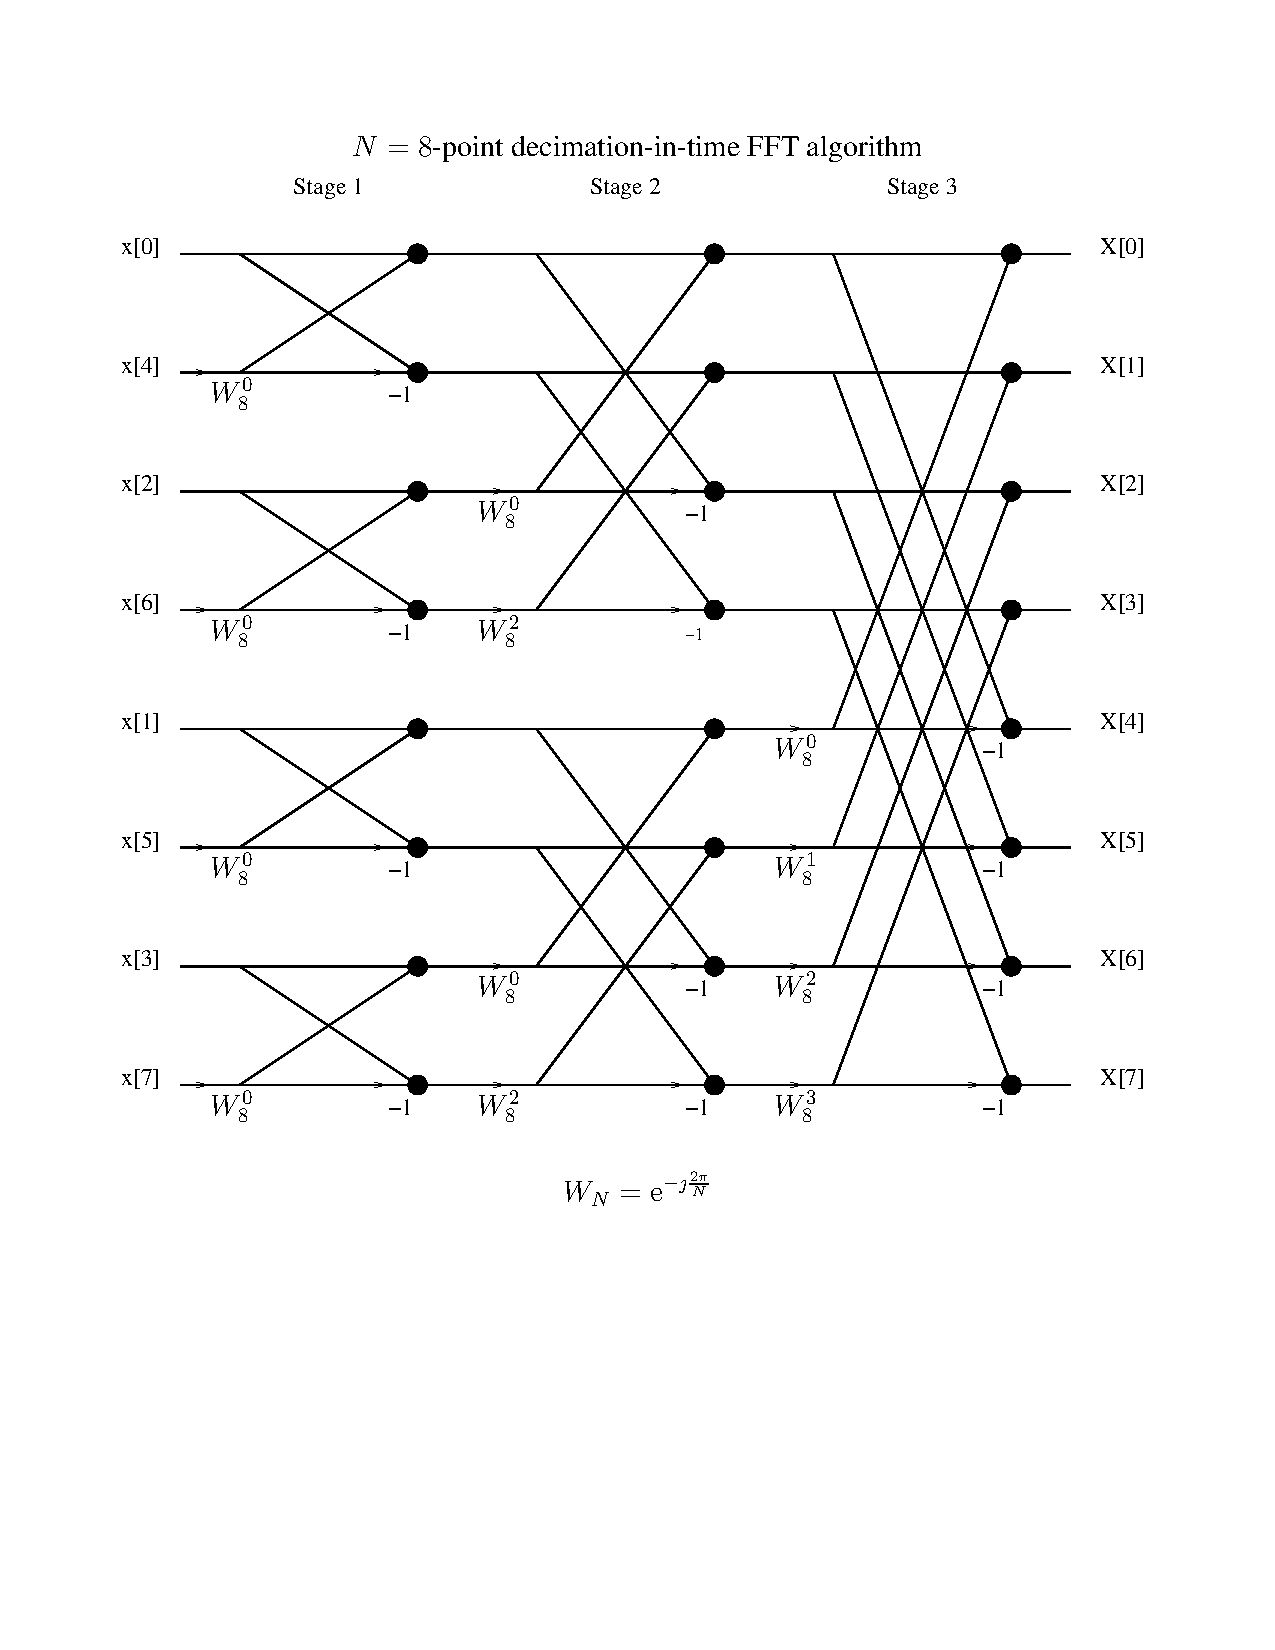
\includegraphics[width=0.65\textwidth]{DITFFT.pdf}
  \end{figure}
 
  
\end{frame}  

%-----------------------------------------------------------------------------------------
\subsection[Danielson-Lanczos Lemma]{Danielson-Lanczos Lemma}
%-----------------------------------------------------------------------------------------
  
\begin{frame}%[shrink=10]
  \frametitle{Danielson-Lanczos Lemma}
  
  The discrete Fourier transform of length $N$ (where $N$ is even) can be rewritten as the \bluebf{sum of two discrete Fourier transforms}, each of length $N/2$, one for \alertbf{even-numbered} points and the other for \alertbf{odd-numbered} points. 
      
  \begin{eqnarray}
    \hat{f}_n	&=&	\frac{1}{\sqrt{2\pi}} \sum_{k=1}^{N} \, f_k  Z_{N}^{nk}	\\
	            &=& \frac{1}{\sqrt{2\pi}} \sum_{k=1}^{N/2} f_{2k} \,  Z_{N/2}^{nk} + Z_N^n \sum_{k=1}^{N/2} Z_{N/2}^{nk} \, f_{2k+1}	\\
	            &=& \hat{f}_n^{\mathrm{even}} + Z_N^n \, \hat{f}_n^{\mathrm{odd}},	
  \end{eqnarray}

  In fact, this procedure can be \bluebf{applied recursively} to break up the $N/2$ even and odd points to their $N/4$ even and odd points. 
  
  \mysp
  
  If $N$ is a power of 2, this procedure breaks up the original transform into $\ln N$ transforms of length 1.
  
\end{frame}  
  
%==========================================================================================
%==========================================================================================
\end{document}
